% !TEX spellcheck = en-US
\chapter{Inertial Sensors}
\label{cha:sensors} 
To combine inertial measurements with additional sensors and models for position and orientation estimation, it is important to accurately describe the quantities measured by the inertial sensors as well as to characterize the typical sensor errors. This will be the topic of this chapter. It will serve as a basis for the probabilistic models discussed in \Chapterref{cha:models}.

As discussed in \Chapterref{cha:introduction}, accelerometers and gyroscopes measure the specific force and the angular velocity, respectively. In~\Sectionref{sec:sensors-angVel} and~\Sectionref{sec:sensors-specForce}, we will discuss these quantities in more detail. To enable a discussion about this, in \Sectionref{sec:sensors-coordFrames} a number of coordinate frames and the transformations between them will be discussed. We assume that we have 3D accelerometers and 3D gyroscopes, \ie that the sensors have three sensitive axes along which these physical quantities are measured. They are measured in terms of an output voltage which is converted to a physical measurement based on calibration values obtained in the factory. Even though the sensors are typically calibrated in the factory, (possibly time-varying) errors can still remain. In \Sectionref{sec:sensors-errors}, the most commonly occurring sensor errors are discussed. 

\section{Coordinate frames}
\label{sec:sensors-coordFrames}
In order to discuss the quantities measured by the accelerometer and gyroscope in more detail, a number of
coordinate frames need to be introduced:
\begin{description}
\item[The body frame $\boldsymbol{b}$] is the coordinate frame of the moving
  \gls{imu}. Its origin is located in the center of the accelerometer
  triad and it is aligned to the casing. All the inertial measurements
  are resolved in this frame.
\item[The navigation frame $\boldsymbol{n}$] is a local geographic frame in which we
  want to navigate. In other words, we are interested in the position and
  orientation of the $b$-frame with respect to this frame. For most
  applications it is defined stationary with respect to the earth. However,
  in cases when the sensor is expected to move over large distances, it is customary to
  move and rotate the $n$-frame along the surface of the
  earth. The first definition is used throughout this tutorial, unless
  mentioned explicitly.
\item[The inertial frame $\boldsymbol{i}$] is a stationary frame. The
  \gls{imu} measures linear acceleration and angular velocity
  with respect to this frame. Its origin is located at the center of the
  earth and its axes are aligned with respect to the stars.
\item[The earth frame $\boldsymbol{e}$] coincides with the $i$-frame, but rotates
  with the earth. That is, it has its origin at the center of the
  earth and axes which are fixed with respect to the earth.
\end{description}
The $n$, $i$ and $e$ coordinate frames are illustrated in \Figureref{fig:sensors-coordinateFrames}. We use a superscript to indicate in which coordinate frame a vector is expressed. Vectors can be rotated from one coordinate frame to another using a rotation matrix. We use a double superscript to indicate from which coordinate frame to which coordinate frame the rotation is defined. An illustration is given in \Exampleref{ex:sensors-rotationVectors}. 

\begin{figure}
	\centering
    	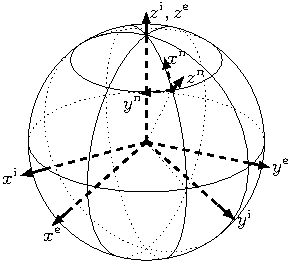
\includegraphics[scale = 1]{figure2_1.pdf}
    	\caption{An illustration of three of the coordinate frames discussed in \Sectionref{sec:sensors-coordFrames}: the $n$-frame at a certain location on the earth, the $e$-frame rotating with the earth
      		and the $i$-frame.}
	\label{fig:sensors-coordinateFrames}
\end{figure}

\begin{myexample}{Rotation of vectors to different coordinate frames}%
\label{ex:sensors-rotationVectors}%
Consider a vector $x$ expressed in the body frame $b$. We denote this vector by $x^\text{b}$. The rotation matrix $R^\text{nb}$ rotates a vector from the body frame $b$ to the navigation frame~$n$. Conversely, the rotation from navigation frame $n$ to body frame $b$ is denoted $R^\text{bn} = ( R^{\text{nb}} )^\Transp$. Hence, the vector $x$ expressed in the body frame ($x^\text{b}$) and expressed in the navigation frame ($x^\text{n}$) are related according to
\begin{align}
x^\text{n} = R^{\text{nb}} x^\text{b}, \qquad x^\text{b} = ( R^{\text{nb}} )^\Transp x^\text{n} = R^{\text{bn}} x^\text{n}.
\end{align}%
\vspace*{-\baselineskip}
\end{myexample}

\section{Angular velocity}
\label{sec:sensors-angVel}
The gyroscope measures the angular velocity of the body frame with respect to the inertial frame, expressed in the body frame~\citep{tittertonW:1997}, denoted by $\omega_{\text{ib}}^\text{b}$. This angular velocity can be expressed as
\begin{align}
\label{eq:sen-imu-gyr-n}
\omega_{\text{ib}}^\text{b}
= R^{\text{bn}} \left(
\omega_{\text{ie}}^\text{n} +
\omega_{\text{en}}^\text{n} \right)
+ \omega_{\text{nb}}^\text{b},
\end{align}
where $R^{\text{bn}}$ is the rotation matrix from the navigation frame to the body frame. The \emph{earth rate}, \ie the angular velocity of the earth frame with respect to the inertial frame is denoted by $\omega_{\text{ie}}$. The earth rotates around its own $z$-axis in $23.9345$ hours with respect to the stars~\citep{nasa:2016}. Hence, the earth rate is approximately $7.29 \cdot 10^{-5}~\radianpersecond$.

In case the navigation frame is not defined stationary with respect to the earth, the angular velocity $\omega_{\text{en}}$, \ie the \emph{transport rate} is non-zero. The angular velocity required for navigation purposes --- in which we are interested when determining the orientation of the body frame with respect to the navigation frame --- is denoted by $\omega_{\text{nb}}$.

\section{Specific force}
\label{sec:sensors-specForce}
The accelerometer measures the specific force $f$ in the body frame $b$~\citep{tittertonW:1997}. This can be expressed as
\begin{align}
\label{eq:sen-imu-acc-i}
f^\text{b} = R^{\text{bn}} 
( a_{\text{ii}}^\text{n} - g^\text{n} ),
\end{align}
where $g$ denotes the gravity vector and $a_{\text{ii}}^\text{n}$ denotes the linear acceleration of the sensor expressed in the navigation frame, which is
\begin{align}
a_{\text{ii}}^\text{n} = R^{\text{ne}} R^{\text{ei}} a_{\text{ii}}^\text{i}.
\end{align}
The subscripts on the linear acceleration $a$ are used to indicate in which frame the differentiation is performed. For navigation purposes, we are interested in the position of the sensor in the navigation frame $p^\text{n}$ and its derivatives as performed in the navigation frame 
\begin{align}
\label{eq:sensors-defva}
\left. \tfrac{\tdiff}{\tdiff t} p^\text{n} \right|_\text{n} = v^\text{n}_\text{n}, \qquad \left. \tfrac{\tdiff}{\tdiff t} v^\text{n} \right|_\text{n} = a^\text{n}_\text{nn}.
\end{align}
A relation between $a_{\text{ii}}$ and $a_{\text{nn}}$ can be derived by using the relation between two rotating coordinate frames. Given a vector $x$ in a coordinate frame $u$,
\begin{align}
\label{eq:sensors-rotatingCF}
\left. \tfrac{\tdiff}{\tdiff t} x^\text{u} \right|_\text{u} = \left. \tfrac{\tdiff}{\tdiff t} R^\text{uv} x^\text{v} \right|_{\text{u}} = R^\text{uv} \left. \tfrac{\tdiff}{\tdiff t} x^\text{v} \right|_{\text{v}} + \omega_{\text{uv}}^\text{u} \times x^\text{u},
\end{align}
where $\omega_{\text{uv}}^\text{u}$ is the angular velocity of the $v$-frame with respect to the $u$-frame, expressed in the $u$-frame. For a derivation of this relation in the context of inertial navigation, see \cite{hol:2011,tittertonW:1997}. For a general introduction, see any textbook on dynamics, \eg \cite{marionT:1995,meriamK:1998}. 

Using the fact that
\begin{align}
p^\text{i} = R^\text{ie} p^\text{e},
\end{align} 
the velocity $v_\text{i}$ and acceleration $a_\text{ii}$ can be expressed as
\begin{subequations}
\label{eq:sensors-pvi-pve}
\begin{align}
v_\text{i}^\text{i} &= \left. \tfrac{\tdiff}{\tdiff t} p^\text{i} \right|_\text{i} = 
\left. \tfrac{\tdiff}{\tdiff t} R^\text{ie} p^\text{e} \right|_\text{i} = 
R^\text{ie} \left. \tfrac{\tdiff}{\tdiff t} p^\text{e} \right|_\text{e} + \omega_{\text{ie}}^\text{i} \times p^\text{i} 
= v^\text{i}_\text{e} + \omega_{\text{ie}}^\text{i} \times p^\text{i}, \\
a_\text{ii}^\text{i} &= \left. \tfrac{\tdiff}{\tdiff t} v^\text{i}_\text{i} \right|_\text{i} = 
\left. \tfrac{\tdiff}{\tdiff t} v^\text{i}_\text{e} \right|_\text{i} + \left. \tfrac{\tdiff}{\tdiff t} \omega_{\text{ie}}^\text{i} \times p^\text{i} \right|_\text{i} \nonumber \\
&= a^\text{i}_\text{ee} + 2 \omega_{\text{ie}}^\text{i} \times v^\text{i}_\text{e} + \omega_{\text{ie}}^\text{i} \times \omega_{\text{ie}}^\text{i} \times p^\text{i},
\end{align} 
\end{subequations}
where we have made use of~\eqref{eq:sensors-defva},~\eqref{eq:sensors-rotatingCF}, and the fact that the angular velocity of the earth is constant, \ie $\tfrac{\tdiff}{\tdiff t} \omega_{\text{ie}}^\text{i} = 0$. Using the relation between the earth frame and the navigation frame 
\begin{align}
p^\text{e} = R^\text{en} p^\text{n} + n_\text{ne}^\text{e},
\end{align} 
where $n_\text{ne}$ is the distance from the origin of the earth coordinate frame to the origin of the navigation coordinate frame, expressions similar to~\eqref{eq:sensors-pvi-pve} can be derived. Note that in general it can not be assumed that $\tfrac{\tdiff}{\tdiff t} \omega_{\text{en}} = 0$. Inserting the obtained expressions into~\eqref{eq:sensors-pvi-pve}, it is possible to derive the relation between $a_\text{ii}$ and $a_\text{nn}$. Instead of deriving these relations, we will assume that the navigation frame is fixed to the earth frame, and hence $R^\text{en}$ and $n_\text{ne}^\text{e}$ are constant and
\begin{subequations}
\label{eq:sensors-pve-pvn}
\begin{align}
v_\text{e}^\text{e} &=
\left. \tfrac{\tdiff}{\tdiff t} p^\text{e} \right|_\text{e} = 
\left. \tfrac{\tdiff}{\tdiff t} R^\text{en} p^\text{n} \right|_\text{e} = 
R^\text{en} \left. \tfrac{\tdiff}{\tdiff t} p^\text{n} \right|_\text{n} = 
v^\text{e}_\text{n}, \\
a_\text{ee}^\text{e} &=
\left. \tfrac{\tdiff}{\tdiff t} v^\text{e}_\text{e} \right|_\text{e} = 
\left. \tfrac{\tdiff}{\tdiff t} v^\text{e}_\text{n} \right|_\text{n} = 
a^\text{e}_\text{nn} .
\end{align} 
\end{subequations}
This is a reasonable assumption as long as the sensor does not travel over significant distances as compared to the size of the earth and it will be one of the model assumptions that we will use in this tutorial. More on the modeling choices will be discussed in \Chapterref{cha:models}. 

Inserting~\eqref{eq:sensors-pve-pvn} into~\eqref{eq:sensors-pvi-pve} and rotating the result, it is possible to express $a_\text{ii}^\text{n}$ in terms of $a_\text{nn}^\text{n}$ as
\begin{align}
\label{eq:sensors-aii-ann} 
a_\text{ii}^\text{n} = 
a_\text{nn}^\text{n} + 
2 \omega_\text{ie}^\text{n} \times v^\text{n}_\text{n} + 
\omega_\text{ie}^\text{n} \times \omega_\text{ie}^\text{n}
\times p^\text{n},
\end{align}
where $a_\text{nn}$ is the acceleration required for navigation
purposes. The term $\omega_\text{ie}^\text{n} \times \omega_\text{ie}^\text{n}
\times p^\text{n}$ is known as the \emph{centrifugal acceleration} and $2 \omega_\text{ie}^\text{n} \times v^\text{n}_\text{n}$ is known as the \emph{Coriolis acceleration}. The centrifugal acceleration is typically absorbed in the (local) gravity vector. In \Exampleref{ex:sensors-magCentrCor}, we illustrate the magnitude of both the centrifugal and the Coriolis acceleration.

\begin{myexample}{Magnitude of centrifugal and Coriolis acceleration}%
\label{ex:sensors-magCentrCor}%
The centrifugal acceleration depends on the location on the earth. It is possible to get a feeling for its magnitude by considering the property of the cross product stating that
\begin{align}
\| \omega_\text{ie}^\text{n} \times \omega_\text{ie}^\text{n} \times p^\text{n} \|_2 \leq 
\| \omega_\text{ie}^\text{n} \|_2 \| \omega_\text{ie}^\text{n} \|_2 \| p^\text{n} \|_2.
\end{align}
Since the magnitude of $\omega_\text{ie}$ is approximately $7.29 \cdot 10^{-5}~\radian\per\second$ and the average radius of the earth is $6371~\kilo\meter$~\citep{nasa:2016}, the magnitude of the centrifugal acceleration is less than or equal to $3.39 \cdot 10^{-2}~\metrepersquaresecond$. 

The Coriolis acceleration depends on the speed of the sensor. Let us consider a person walking at a speed of $5~\kilo\meter\per\hour$. In that case the magnitude of the Coriolis acceleration is approximately $2.03 \cdot 10^{-4}~\metrepersquaresecond$. For a car traveling at $120~\kilo\meter\per\hour$, the magnitude of the Coriolis acceleration is instead $4.86 \cdot 10^{-3}~\metrepersquaresecond$. 
\end{myexample}

\section{Sensor errors}
\label{sec:sensors-errors}
As discussed in \Sectionref{sec:sensors-angVel} and~\Sectionref{sec:sensors-specForce}, the gyroscope measures the angular velocity $\omega^\text{b}_\text{ib}$ and the accelerometer measures the specific force $f^\text{b}$. However, as already briefly mentioned in \Sectionref{sec:intro-imusForPose}, there are several reasons for why this is not exactly the case. Two of these reasons are a slowly time-varying sensor bias and the presence of measurement noise. The sensor errors in the inertial measurements are illustrated in \Exampleref{ex:sensors-inertialMeasurements} using experimental data. 

\newpage 

\begin{myexample}{Inertial sensor measurements and their errors}%
\label{ex:sensors-inertialMeasurements}%
In Figures~\ref{fig:sensors-accgyrMeas}--\ref{fig:sensors-accMeasNoiseHist}, gyroscope and accelerometer measurements are displayed for around $10$ seconds of stationary data collected with a Sony Xperia Z5 Compact smartphone. Since the smartphone is stationary, the gyroscope is expected to only measure the earth's angular velocity. However, as can be seen in \Figureref{fig:sensors-gyrMeas}, the gyroscope measurements are corrupted by noise. As shown in \Figureref{fig:sensors-gyrMeasNoiseHist}, this noise can be seen to be quite Gaussian. Furthermore, the measurements can be seen to be biased. 

During the stationary period, we would expect the accelerometer to measure the gravity, the centrifugal acceleration and the Coriolis acceleration. Note that again the measurements are corrupted by noise, which can be seen to be quite Gaussian in \Figureref{fig:sensors-accMeasNoiseHist}. The $x$- and $y$-components of the accelerometer measurements are not zero-mean. This can be due to the fact that the table on which the smartphone lies is not completely flat, implying that part of the gravity vector is measured in these components. It can also reflect a sensor bias. The $z$-component is actually larger than expected which indicates the presence of an accelerometer bias at least in this axis. 

Note that from the above discussion it can be concluded that it is more straightforward to determine the gyroscope bias than it is to determine the accelerometer bias. To be able to estimate the gyroscope bias, it is sufficient to leave the sensor stationary. For the accelerometer, however, it is in that case difficult to distinguish between a bias and a table that is not completely flat. For more information about accelerometer or general inertial sensor calibration, see~\cite{tedaldiPM:2014,olssonKHS:2016,panahandehSJ:2010}. 

The gyroscope in the smartphone is automatically recalibrated during stationary time periods. The measurements shown in \Figureref{fig:sensors-gyrMeas} have not been corrected for this (so-called uncalibrated or raw data). The reason why the gyroscope is calibrated during stationary periods, is because its bias is slowly time-varying. As an example, let us consider a data set of $55$ minutes. The gyroscope bias during the first minute of the data set was $\begin{pmatrix} 35.67 & 56.22 & 0.30 \end{pmatrix}^\Transp \cdot 10^{-4}~\radianpersecond$, while the gyroscope bias during the last minute of the data set was $\begin{pmatrix} 37.01 & 53.17 & -1.57 \end{pmatrix}^\Transp \cdot 10^{-4}~\radianpersecond$.

\begin{figure}
	\centering
	\subfigure[Gyroscope measurements $y_{\omega,t}$ which we expect to consist only of the earth's angular velocity.]{
	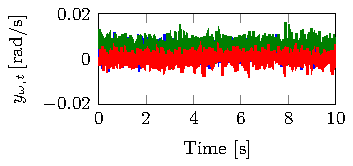
\includegraphics[scale = 1]{figure2_2a.pdf}
	\label{fig:sensors-gyrMeas}} 
	\tikzsetnextfilename{sensors-accMeas}
	\subfigure[Accelerometer measurements $y_{\text{a},t}$ which we expect to consist of the gravity vector, the centrifugal acceleration and the Coriolis acceleration.]{
	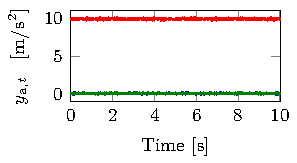
\includegraphics[scale = 1]{figure2_2b.pdf}
	\label{fig:sensors-accMeas}} 
    	\caption{Inertial measurements for $10$ seconds of stationary data. As can be seen, the measurements are corrupted by noise and have a bias.}
	\label{fig:sensors-accgyrMeas}
\end{figure}

\begin{figure}
	\centering
    	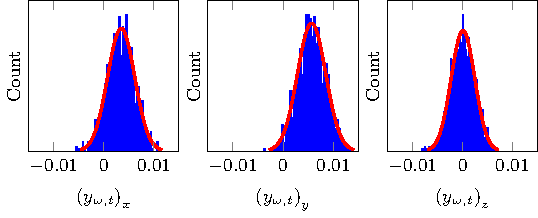
\includegraphics[scale = 1]{figure2_3.pdf}
    	\caption{Histogram (blue) of the gyroscope measurements for $10$ seconds of data from a stationary sensor and a Gaussian fit (red) to the data. As can be seen, the measurement noise looks quite Gaussian.}
	\label{fig:sensors-gyrMeasNoiseHist}
\end{figure}

\begin{figure}
	\centering
    	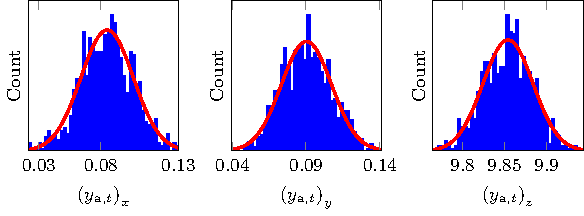
\includegraphics[scale = 1]{figure2_4.pdf}
    	\caption{Histogram (blue) of the accelerometer measurements for $10$ seconds of data from a stationary sensor and a Gaussian fit (red) to the data. As can be seen, the measurement noise looks quite Gaussian. Note the different scales on the horizontal axis.}
	\label{fig:sensors-accMeasNoiseHist}
\end{figure}
\end{myexample}

The performance of \glspl{imu} is often specified in terms of their \emph{Allan variance} \citep{ieeeStd1559:2009,elsheimy:2008,allan:1966}. The Allan variance gives information about the sensor errors for stationary conditions, \ie in a stable climate without exciting the system. It studies the effect of averaging measurements for different \emph{cluster times} $T_c$. Typically, the Allan \emph{standard deviation} $\sigma_\text{A}(T_c)$ is plotted against the cluster time $T_c$ as illustrated in \Figureref{fig:sensors-allanVariance}. This figure shows the characteristic behavior of the Allan variance for inertial sensors. To study it more in detail, we will discuss two components of the Allan variance that are typically of concern for inertial sensors: the white noise and the bias instability. 

\begin{figure}
	\centering
    	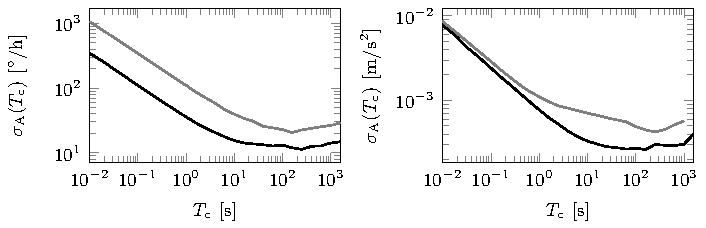
\includegraphics[scale = 1]{figure2_5.pdf}
    	\caption{Left: Allan deviation for two gyroscopes. Right: Allan deviation for two accelerometers. Reproduced with permission from~\cite{vydhyanathanBLS:2015}.}
	\label{fig:sensors-allanVariance}
\end{figure}

Assume, as in \Exampleref{ex:intro-integrationDrift}, that we have a white noise signal with standard deviation $\sigma$. A longer averaging time would for this signal lead to values closer to zero. The contribution to the Allan standard deviation from the white noise component is given by $\sigma_\text{A}(T_c) = \tfrac{\sigma}{\sqrt{n}}$ where $n$ is the number of samples averaged over. This corresponds to a line with slope $-1/2$ in a $\log$--$\log$ plot. For instance in the Allan deviation for the gyroscope in \Figureref{fig:sensors-allanVariance}, the lines can be seen to have a slope of $-1/2$ until around $10-20~\second$, which indicates that the white noise is the dominating source of error for these short integration times. 

A constant bias does not have any effect on the Allan variance diagram. However, in case the bias changes, longer averaging times will no longer be beneficial. Hence, the Allan variance diagrams in \Figureref{fig:sensors-allanVariance} show a deviation from the slope $-1/2$ for longer averaging times. 

The Allan variance is a useful tool to study and compare the noise characteristics of inertial sensors. However, it only considers stationary conditions. In dynamic conditions, a large number of other error sources potentially come into play, see \eg \cite{tittertonW:1997,woodman:2007}. These are for instance related to the fact that the sensors sample at discrete times. Hence, to capture high-frequency signals, high sampling frequencies are desired~\citep{savage:1998a,savage:1998b}. Furthermore, large dynamics can lead to erroneous or saturated measurements. Other errors that are not included are for instance changes in the sensitivity of the axes due to changes in temperature. We should therefore never just rely on the Allan variance when deciding which sensor to use in a particular application.